%%
%% Copyright Guy Taylor 2012
%%
%%

\chapter{Implementation and Testing}

\section{Development Environment}
Unlike traditional desktop development where the development code, compiler
and debugger are present on the same system, in embedded development the
roles are split across three devices. These systems are also mostly unstandardised
and need proprietary devices or software to function. Achieving a stable and
effective development environment enables more agile development and
helps assist rather than inhibit the programmer.

\subsection{\acf{IDE}}
I initially used the free ARM MDK IDE because it was being used in a concurrent Respire Project. I
found MDK to be unsatisfactory for my needs and moved mid-project to the Eclipse \ac{IDE}, which is
one of the leading \acp{IDE} in the embedded development field, and in many others. I chose it because it
is fast becoming the industry standard and is being used as the basis for official ARM MD5 IDE.
Eclipse is also both open source and fully supported on Linux, enabling use without cost for this
project.

\subsection{Compiler}
The ARM Compiler tool chain (previously known as ARM RealView Compilation) used during the
initial stages. I transitioned to the \ac{GCC} during development to both
prevent vendor lock-in and enable the use of Linux as the host development environment. \ac{GCC} was
used in the final and most successful development setup, superseding the ARM compiler which only
works on Windows\textregistered and is not fully supported using the \ac{GDB} backend. The \ac{GCC} compiler supports
a much larger number of processor targets, is available free of charge and is supported on both
Windows\textregistered and Linux. \ac{GCC} is also fully supported by \ac{GDB} and Eclipse. Specifically, I used Mentor
Graphics' Sourcery CodeBench Lite Edition (formally Sourcery G++), a branch of \ac{GCC} dedicated to
migrating the optimisation skew away from the x86 instruction set to the ARM family.
The use of the compiler's pre-processor was core to the ability to enable a clean single code base
and remove unneeded runtime calculations. Many of the configuration settings were programmed
via the pre-processor and so could allow the user to reconfigure the system without reviewing
complex data sheets.
{inset code snippet}


\subsection{Debugger}
To achieve the aims of reducing vendor lock-in and provide a better environment to program in, the
\ac{GDB} was chosen. The \ac{GDB} platform is the reference implementation of a
separated front and back end debugging system and the Mentor Graphics branch of this project was
utilised to best interact with the chosen compiler.

\begin{wrapfigure}{r}{0.6\textwidth}
  \vspace{-10pt}
  \begin{center}
    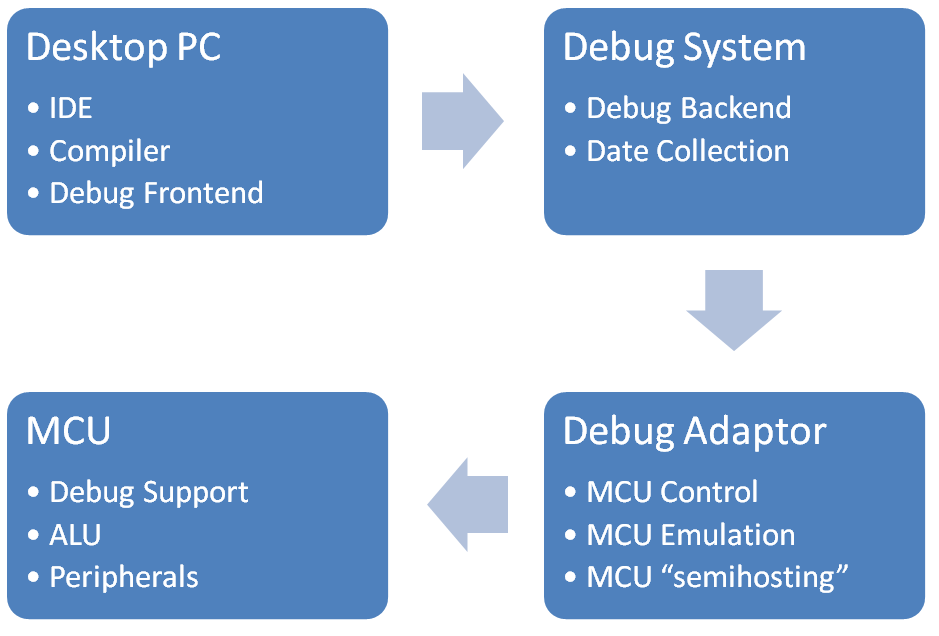
\includegraphics[width=0.5\textwidth, keepaspectratio=true]{images/debug_system.png}
  \end{center}
  \caption[Debug System Architecture]{Debug System Architecture}
  \vspace{-10pt}
\end{wrapfigure}

The debugging backend is highly coupled with the debugging emulator hardware adaptor used in the
project. The Energy Micro development boards used have an embedded SEGGER J-Link debugger
and therefore a SEGGER J-Link EDU debugger was chosen for consistency when an additional
debugging device was needed. The J-Link platform was chosen as it is well supported by Energy
Micro, works with GDB on both Windows(r) and Linux and supports the needed features. The Open
On-Chip Debugger project was tested but found to be too immature in its SWD debugging support,
as it could not correctly debug the system.


For additional ease of use, I produced a GDB proxy to implement a SWO viewer and work around
issues as they arose. A Python TCP GDB proxy was produced as the project continued and new
features were needed, which included:-
\begin{itemize}
  \item Managing multiple GDB connections to a single backend. The system will cleanly terminate
        the current connection allowing the new connection to take over. This is important as it
        prevents the Eclipse debugger from freezing for minutes at a time.
  \item Viewing of the raw GDB communications. Important in diagnosing the location of
        problematic events within the long opaque chain of systems.
  \item Displaying SWO output when enabled, separating the different types of information (e.g.
        printf, interrupts and timings). For the project environment using GDB, the system was
        unable to read live SWO output due to the SEGGER GDB server not passing the values on.
\end{itemize}


Integrating the powerful Eclipse debugging tool into this system allowed live code changes to be
made on the device as well as a clean GUI, enabling single stepping, expressions, variables and
advanced break point functions to be managed.


At the hardware level, I produced a 20pin JTAG/SWO connector to the 9pin Respire header. This
allowed quick insertion and removal of connectors without damaging the fragile header pins, whilst
also regulating the 5Volts supply to the required 3.3Volts. A small circuit was also produced to
enable error-free monitoring of SPI communications.

% TODO
{insert pic}


\subsection{Digital Logic Probe}

\begin{wrapfigure}{r}{0.6\textwidth}
  \vspace{-10pt}
  \begin{center}
    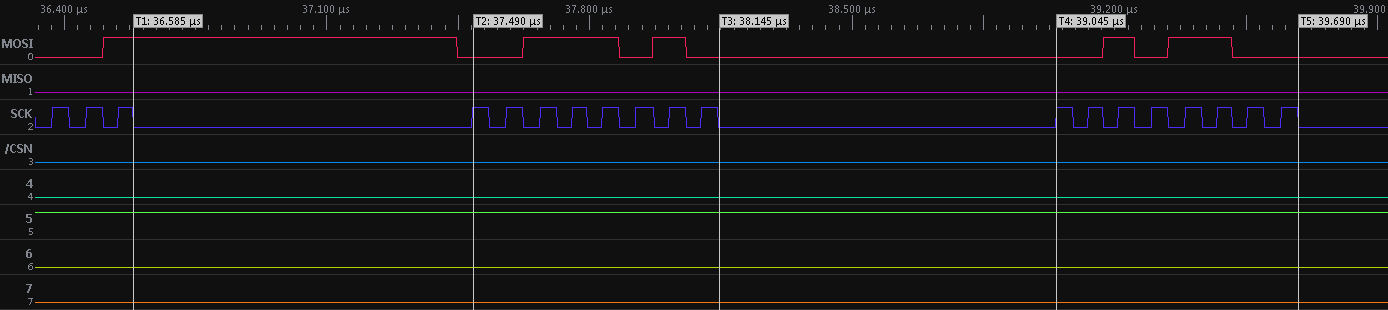
\includegraphics[width=0.5\textwidth, keepaspectratio=true]{images/digital_probe.png}
  \end{center}
  \caption[Digital Probe Trace]{Digital Probe Trace}
  \vspace{-10pt}
\end{wrapfigure}

Throughout the project implementation, it was important to be able to view the communications,
states and timings of the devices pins. To achieve this, an Open Bench Logic Sniffer digital probe was
used as it allowed:
\begin{itemize}
  \item The high accuracy of timing required, down to 5 nanoseconds.
  \item Automated decoding of SPI communication when linked to the Logic Sniffer software.
  \item Automated frequency and duty cycle calculations with error calculations.
  \item Multiple trigger configurations so only the required data was collected, enabling higher
        sampling rates.
\end{itemize}

\subsection{Developmental Hardware}
Throughout development, I used two EFM32-SDK development boards produced by the processor
manufacturer (Energy Micro HA) and a specially-adapted Respire unit which had a replacement
connection between the LETIMER and the NRF24 radio (inseret pin x and y; produced by J. Mann at
my request). This equipment was sufficient to test a 3-node network.

\section{Firmware}

\subsection{Nested Vector Interrupt Controller}
The Nested Vector Interrupt Controller (NVIC) of the Cortex-M3 was used to allow the system to be
more predictable. Given the event-driven design of my implementation, there is a higher risk of
interrupt coincidence, increasing delays in time-critical sections of code. To combat this potential
issue, I gave each interrupt a priority to allow the advanced interrupt controller to reorder the
interrupts.

{code nippet of NVIC SetPriority}

In many interrupts, I also chose to release the interrupt lock early to prevent missed events. This was
carefully planned in each occurrence as misuse of the feature can cause an infinite interrupt loop.
This more complex system was chosen as it works in bursts suitable for TDMA, with multiple time-
critical sections condensed together.


{code snippet to show interrupt reset}


I also utilised the Cortex-M3s SysTick feature in combination with the interrupt system to enable a
power efficient delay function for delays over 2msec.
{code snippet}


\subsection{Events and Interrupts}
Throughout the code base, I made extensive use of \acf{WFI}, \acf{WFE} and \acf{SEV}
which are allowable in the Cortex-M3. These instructions set extensions,
facilitate reducing the inefficient nature of polling for change. The common implementation of the
'while-loop' polling for a required change of state prevents the system from powering down. By
using the above instructions correctly, I aimed to power down the system without introducing
latency, by configuring the loops to exit after an interrupt where appropriate.
{insert graph}


In events where a software interrupt was required, I used the SEV instruction, SEVs are more
efficient than interrupts for this purpose as they do not have an Interrupt Service Routine (ISR)
connected to their behaviour.


{insert code snippet}


\subsection{Peripheral Reflex System (PRS)}
\label{sec:PRS}
The \ac{PRS} unique to the EFM32 enabled me to implement a novel system to reduce the duty cycle.
This requires synchronisation of \ac{RTC} on all devices sharing a common frequency. I
configured the \ac{RTC} and the \ac{LETIMER} on each device using \ac{PRS} such that an \ac{RTC}
pulse initiates the following sequence of events in each device at the beginning of every \ac{TDMA} cycle
(of length specified in the network design):-
\begin{enumerate}
  \item The NRF24 enable pin is briefly pulsed on all devices (preconfigured where Respires are in
        Receive mode and Base Stations are in Transmit mode)
  \item The NRF24 enable pin is toggled on in the Base Station (in Receive mode)
  \item The NRF24 enable pin on each Respire device is pulsed sequentially (in Transmit mode) as
        determined by its unique network address
  \item The NRF24 enable pin on the Base Station is toggled off.
\end{enumerate}


This recurrent sequence is illustrated in Figure ZZ. The EFM32 microcontroller remains in a low-energy
state throughout each sequence, except for interrupts from the \ac{LETIMER} (configured to
trigger when the \ac{NRF24} enable pin switches off) or the radio (on receipt or transmission of packet)
within the network section of the code.


Insert diagram here


During implementation of this system I encountered difficulties when enabling the \ac{PRS} to coordinate
the \ac{RTC} and \ac{LETIMER} triggers, which had both worked independently. After further
research and analysis, it was discovered that the \ac{RTC} and \ac{LETIMER} are required to have the same
periodicity for this \ac{PRS} configuration. I chose to increase the \ac{RTC} period (away from the most
efficient value) to match that required by the \ac{LETIMER}, which resulted in an insignificant power
increase which was likely to be far outweighed by the power efficiency gains of the \ac{PRS}. (numbers
required)

\subsection{Implementation of Firmware Modules}
The Firmware was implemented to the design of Figure X by incorporating the modules and systems
described below.

\begin{wrapfigure}{r}{0.6\textwidth}
  \vspace{-10pt}
  \begin{center}
    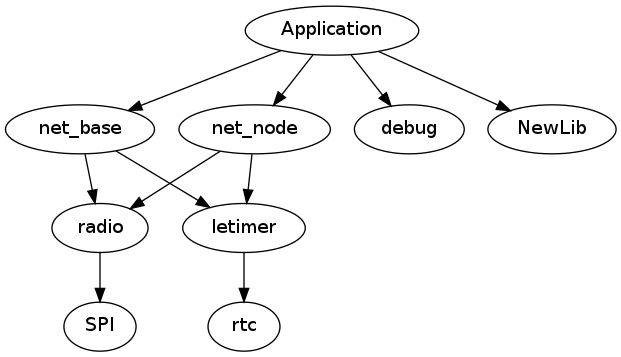
\includegraphics[width=0.5\textwidth, keepaspectratio=true]{images/modules_dep.png}
  \end{center}
  \caption[System Architecture]{System Architecture}
  \vspace{-10pt}
\end{wrapfigure}

\subsubsection{Serial Peripheral Interface (SPI)}
An initial baud rate of 1MHz was chosen to coincide with the Energy Micro application notes. At
1MHz the \ac{SPI} \ac{USART} runs at 10\% of the NRF24's maximum and 7\% of the EFM32's maximum (using
the current clock speed). At this rate, a successful 32byte packet and 2 byte command upload to the
radio took 150msec. In an attempt to improve the performance and reduce the duty cycle of the
system, I investigated whether increasing the \ac{SPI} baud rate alone would help because the period of
many of the system events in the highest power states is dependent on the speed of data that can
be transferred to and from the \ac{NRF24}. However, it was found that increasing the baud rate to 7MHz
(the EFM32 maximum) made no improvement.

After analysis using the digital probe (ref fig z.) it was found that although the period taken for each
byte decreased, the period between byte transmission did not change. This suggested that the \ac{MCU}
was unable to sustain transfer with only a single buffer (note that a race condition may occur
without correct flushing of the transmit buffer due to an incorrect Chip Select Pin state). A fix was
attempted by the use of the double hardware buffer but I was unsuccessful due to a hardware flaw
in the EFM32 (ref needed).


\subsubsection{DataLink Module}
This module initialises and configures the \ac{NRF24} radio, uploads and downloads the packet data from
the network modules to the radio and manages radio power and state.

\begin{figure}
  \vspace{-10pt}
  \begin{center}
    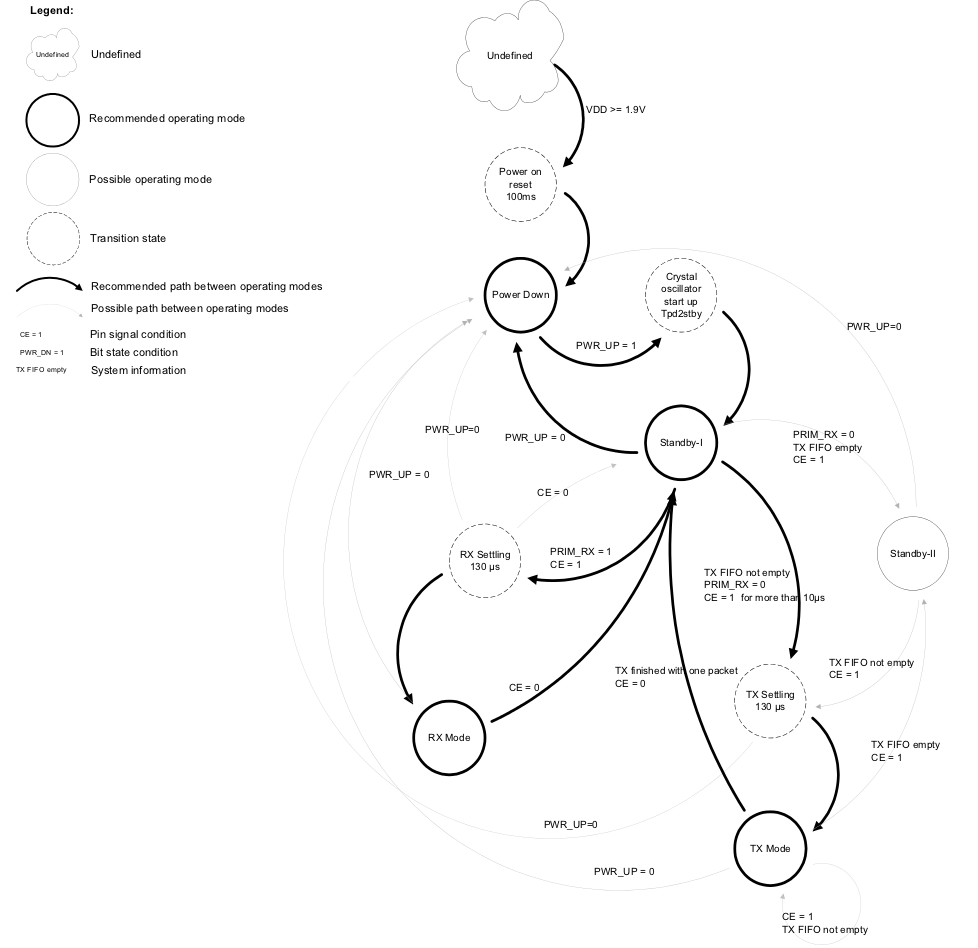
\includegraphics[width=0.9\textwidth, keepaspectratio=true]{images/nrf24_state.png}
  \end{center}
  \caption[\ac{NRF24} State Machine]{\ac{NRF24} State Machine \cite{NRF24Spec}}
  \vspace{-10pt}
\end{figure}

Insert code snippet


Insert table


During development it was found that there were many issues related to the correct
communication, state control, and timing of the \ac{NRF24} radio. Throughout development, consistent
issues arose concerning the radio as it did not perform as suggested by the device documentation.
During discussions with the designer of the Respire, Janick Mann, several interpretations of the
NRF24 specification were considered. Several simple test applications were implemented using 4
separate \ac{NRF24} radios on 2 different EFM32 development boards. One such test configured the
radio to broadcast an unmodulated carrier signal, the manufacturer’s recommended testing method
(Ref Constant carrier wave output for testing) which required specialized radio spectrum analysers
to detect and analyse the signal. Initially the \ac{NRF24} hardware was found to behave as expected, but
when more complex interactions with the radio were tested (e.g. a ping-pong firmware application)
the receive-transmit functions became problematic and no reliable solution was found.
Furthermore, during this testing we discovered that high frequency changes exacerbated the issue
and unfortunately high frequency transitioning is required for \ac{TDMA}. Both myself and Janick Mann
concluded that the most plausible cause of this problem was due to the \ac{NRF24} entering the
'standby- II' state. Within this state it is only possible to transition to a receive state through a
lengthy reset process or by transmitting a new packet (which is unacceptable for \ac{TDMA}). Several
modifications of the firmware were produced attempting either to prevent the \ac{NRF24} entering the
'standby- II' state or to progress it out of this state through a reset procedure. No permanent
solution was found within the time constraints of this project.


\subsubsection{Network Modules}
An initial implementation of both \ac{MCU} and the lower power \ac{PRS} systems were produced but these
could not be adequately tested to the required levels because of the problems described above.


\subsubsection{\acf{RTC}}
The EFM32 has a built in 24-bit \ac{RTC} connected to the Respire’s 32.768KHz external
clock and so it was decided to use this to ensure that the system kept good time. I configured the
system to provide a clock reference down to 30.518 μseconds (discussed in \ref{sec:PRS}). This
implementation will also track time over successive RTC overflow events every 1.52days and
minimises interrupts from low-power states.


\subsubsection{SysTick}
The SysTick feature of the Cortex-M3 enables a dedicated priority interrupt connected to the MCU
clock. By setting an appropriate prescaler to the SysTick, a predictable periodic interrupt is created.
This periodic 'tick' is aimed at supporting pre-emptive \ac{RTOS}\cite{RTOS2011} but for this project
it was utilised to produce a more efficient delay function.


In low-power systems, any delay run on the MCU should be avoided, as it wastes power on 'empty'
cycles. However during firmware development, this feature is highly desirable. To enable delays with
power efficiency in mind, the SysTick was used to allow 1msecond increments of the delay to be run
in a lower energy state.

\begin{figure}
  \vspace{-10pt}
  \begin{center}
    \lstset{language=[ANSI]C}
    \begin{lstlisting}
void Delay(uint32_t dlyTicks) {
  uint32_t curTicks;
  curTicks = msTicks;
  while ((msTicks - curTicks) < dlyTicks) ;
}

/* delay 10ms */
delay(10);
    \end{lstlisting}
    \caption[ToDo]{ToDo\cite{EFM32STK}}
  \end{center}
  \vspace{-10pt}
\end{figure}

By utilising the Energy Micro's Energy Profiler, I discovered that the example SysTick function
provided by Energy Micro was negatively impacting on the duty cycle. By modifying this function to
enabling the SysTick only during delays, I produced an effective solution to overcome this issue
without having to sacrifice the lower power delay.


\begin{figure}
  \vspace{-10pt}
  \begin{center}
    \lstset{language=[ANSI]C}
    \begin{lstlisting}
void Delay(uint8_t dlyTicks) {
  uint8_t till;
  /* Setup SysTick Timer for 1 msec interrupt  */
  SysTick_Config((SystemCoreClock/HFRCO_FREQUENCY)*1000);
  till = (msTicks + dlyTicks);
  while (msTicks != till) {
    __WFI();
  }
  SysTick->CTRL = 0x00;
  NVIC_DisableIRQ(SysTick_IRQn);
}
    \end{lstlisting}
    \caption[ToDo]{ToDo\cite{EFM32STK}}
  \end{center}
  \vspace{-10pt}
\end{figure}

\subsubsection{Debug}
I implemented a debug module on the device to assist in the development process. This included full
support for interacting with the digital probe to produce and test accurate timings and
communications. I also developed an extended version of the Energy Micro \ac{SWO} code to add
support for printing to the console of the development PC, linked to the produced \ac{SWO} viewer.

\begin{figure}
  \vspace{-10pt}
  \begin{center}
    \lstset{language=[ANSI]C}
    \begin{lstlisting}
/**
 * Support a 'file system'.
 * printf and related functions depend on this.
 */
int _write(int file, char *ptr, int len) {
  switch (file) {
  case STDOUT:
    i = len;
    while (i--) {
      ITM_SendChar(*ptr++);
    }
    return len;
  break;
  default:
    return -1;
  }
}

/* Print through the debugger */
write(STDOUT, "This helps debugging\n", 21);
    \end{lstlisting}
    \caption[printf Support]{printf Support}
  \end{center}
  \vspace{-10pt}
\end{figure}

\subsubsection{Newlib Library}
Newlib is a small standard C library designed for use in embedded \acp{MCU}. With the C language there
is a standard core library of functions that allow the programmer to maintain code portability. The
use of many of these functions however are application specific in \acp{MCU} (\eg where should the
console go and how to query the device for the time?) and therefore need to be written for the
device used. Newlib is a collection of many optimised implementations for a large number of
platforms, however it did not have specific functions for the EFM32. I chose to implement a subset
of these functions to allow the use of advanced features such as dynamic memory (\ie malloc). The
choice of Newlib was made as it already included a core set of features generic to all Coretx-M3
processors and was the library supported by the compiler.

\begin{figure}
  \vspace{-10pt}
  \begin{center}
    \lstset{language=[ANSI]C}
    \begin{lstlisting}
static unsigned char heap[HEAP_SIZE];
static unsigned char *heap_end = heap;
/**
 * Increase program data space.
 * malloc and related functions depend on this.
 */
caddr_t _sbrk(int incr) {
  unsigned char *prev_heap_end;
  prev_heap_end = heap_end;
  if (heap_end - heap + incr > HEAP_SIZE) {
    write(STDOUT, "Heap overflow\n", 14);
    abort();
  }
  heap_end += incr;
  return (caddr_t) prev_heap_end;
}

/* malloc and free */
free(malloc(1));
    \end{lstlisting}
    \caption[printf Support]{printf Support}
  \end{center}
  \vspace{-10pt}
\end{figure}

